%%%%%%%%%%%%%%%%%%%%%%%%%%%%%%%%%%%%%%%%%%%%%%%%%%%%%%%%%%%%%%%%%%%%%%%%%%%%
%% Author template for INFORMS Journal on Data Science (ijds) [interim solution; new styles under construction]
%% Mirko Janc, Ph.D., INFORMS, mirko.janc@informs.org
%% ver. 0.91, March 2015 - updated November 2020 by Matthew Walls, matthew.walls@informs.org
%% Adapted for rticles by Rob J Hyndman Rob.Hyndman@monash.edu. Dec 2021
%%%%%%%%%%%%%%%%%%%%%%%%%%%%%%%%%%%%%%%%%%%%%%%%%%%%%%%%%%%%%%%%%%%%%%%%%%%%
\documentclass[,ijds,nonblindrev]{informs}

\OneAndAHalfSpacedXI
%%\OneAndAHalfSpacedXII % Current default line spacing
%%\DoubleSpacedXII
%%\DoubleSpacedXI

%% BEGIN MY ADDITIONS %%
\usepackage{hyperref}

% tightlist command for lists without linebreak
\providecommand{\tightlist}{%
  \setlength{\itemsep}{0pt}\setlength{\parskip}{0pt}}



\usepackage{graphicx}
\usepackage{caption}
\setlength{\parindent}{0pt}
\setlength{\parskip}{1em}
\usepackage{booktabs}
\usepackage{multirow}
\usepackage{booktabs}
\usepackage{tabularx}
\usepackage{graphicx}
\usepackage{makecell}
\usepackage{float}
\usepackage{tikz}
\usepackage{siunitx}
\usepackage{tablefootnote}
\usepackage{longtable}
\usepackage{threeparttable}
\usepackage{natbib}
\usepackage{caption}
\usepackage{adjustbox}
\usepackage{multirow}
\usepackage[]{mdframed}

%% END MY ADDITIONS %%


% Natbib setup for author-year style
\usepackage{natbib}
 \bibpunct[, ]{(}{)}{,}{a}{}{,}%
 \def\bibfont{\small}%
 \def\bibsep{\smallskipamount}%
 \def\bibhang{24pt}%
 \def\newblock{\ }%
 \def\BIBand{and}%


%% Setup of theorem styles. Outcomment only one.
%% Preferred default is the first option.
\TheoremsNumberedThrough     % Preferred (Theorem 1, Lemma 1, Theorem 2)
%\TheoremsNumberedByChapter  % (Theorem 1.1, Lema 1.1, Theorem 1.2)
\ECRepeatTheorems

%% Setup of the equation numbering system. Outcomment only one.
%% Preferred default is the first option.
\EquationsNumberedThrough    % Default: (1), (2), ...
%\EquationsNumberedBySection % (1.1), (1.2), ...

% For new submissions, leave this number blank.
% For revisions, input the manuscript number assigned by the on-line
% system along with a suffix ".Rx" where x is the revision number.
\MANUSCRIPTNO{to be added later}

%%%%%%%%%%%%%%%%
\begin{document}
%%%%%%%%%%%%%%%%

% Outcomment only when entries are known. Otherwise leave as is and
%   default values will be used.
%\setcounter{page}{1}
%\VOLUME{00}%
%\NO{0}%
%\MONTH{Xxxxx}% (month or a similar seasonal id)
%\YEAR{0000}% e.g., 2005
%\FIRSTPAGE{000}%
%\LASTPAGE{000}%
%\SHORTYEAR{00}% shortened year (two-digit)
%\ISSUE{0000} %
%\LONGFIRSTPAGE{0001} %
%\DOI{10.1287/xxxx.0000.0000}%

% Author's names for the running heads
% Sample depending on the number of authors;
\RUNAUTHOR{%
true
}
% \RUNAUTHOR{Jones and Wilson}
% \RUNAUTHOR{Jones, Miller, and Wilson}
% \RUNAUTHOR{Jones et al.} % for four or more authors
% Enter authors following the given pattern:
%\RUNAUTHOR{}

\RUNTITLE{ERPO Laws and Firearm Suicide}

\TITLE{Effectiveness of Extreme Risk Protection Orders on Firearm
Suicide}

\ARTICLEAUTHORS{%
\AUTHOR{Jacob Jameson}
\AFF{Harvard Kennedy School, Harvard
University, \EMAIL{\href{mailto:jacobjameson@g.harvard.edu}{\nolinkurl{jacobjameson@g.harvard.edu}}}}

%
}

\ABSTRACT{\textbf{Background:} Extreme Risk Protection Orders (ERPOs),
also known as ``red flag laws,'' allow law enforcement or family members
to petition a court to temporarily remove firearms from individuals
deemed to pose a risk to themselves or others. Although ERPO laws are
designed to prevent firearm-related harm, evidence on their
population-level impact on suicide rates remains limited.

\textbf{Methods:} We conducted a state-year panel analysis using a
Bayesian autoregressive model to evaluate the effect of ERPO enactment
on firearm suicide rates among adults in the United States from 2000 to
2022. Our primary outcome was the state-level annual firearm suicide
rate, stratified by sex and age group.

\textbf{Results:} ERPO implementation was associated with a posterior
mean reduction in firearm suicide rates of X per 100,000 population
(95\% credible interval: Y--Z) among adult men, with no significant
change among women. Sensitivity analyses adjusting for time-varying
state-level covariates and model specifications yielded consistent
findings.

\textbf{Conclusions:} ERPO laws may be effective in reducing firearm
suicide rates, particularly among men. These findings support the
continued expansion and enforcement of ERPO legislation as part of a
comprehensive suicide prevention strategy.}

\KEYWORDS{firearm suicide; ERPO; Bayesian modeling; causal
inference; state policy evaluation}

\maketitle


\section{Introduction}\label{introduction}

Firearm suicide is a major public health crisis in the United States,
accounting for more than half of all suicide deaths each year. Men
constitute the vast majority of firearm suicide decedents, and the
lethality of firearms makes attempts with guns far more likely to result
in death than other methods.

Extreme Risk Protection Orders (ERPOs) have emerged as a promising legal
mechanism to temporarily restrict firearm access for individuals deemed
at imminent risk of harm to themselves or others. These civil orders,
enacted in more than 20 states, are designed to interrupt escalating
risk---particularly for individuals experiencing suicidal crises. While
case reports and early evaluations have suggested that ERPOs may be
effective in averting imminent suicide attempts, population-level
evidence on their longer-term effects remains limited and contested.

In this study, we use a Bayesian state-year panel model to evaluate the
effect of ERPO laws on firearm suicide rates. Our analysis spans over
two decades and includes all 50 U.S. states and the District of
Columbia. We hypothesize that the implementation of ERPO laws is
associated with a measurable reduction in firearm suicide, particularly
among men.

\begin{figure}[t] 
\centering
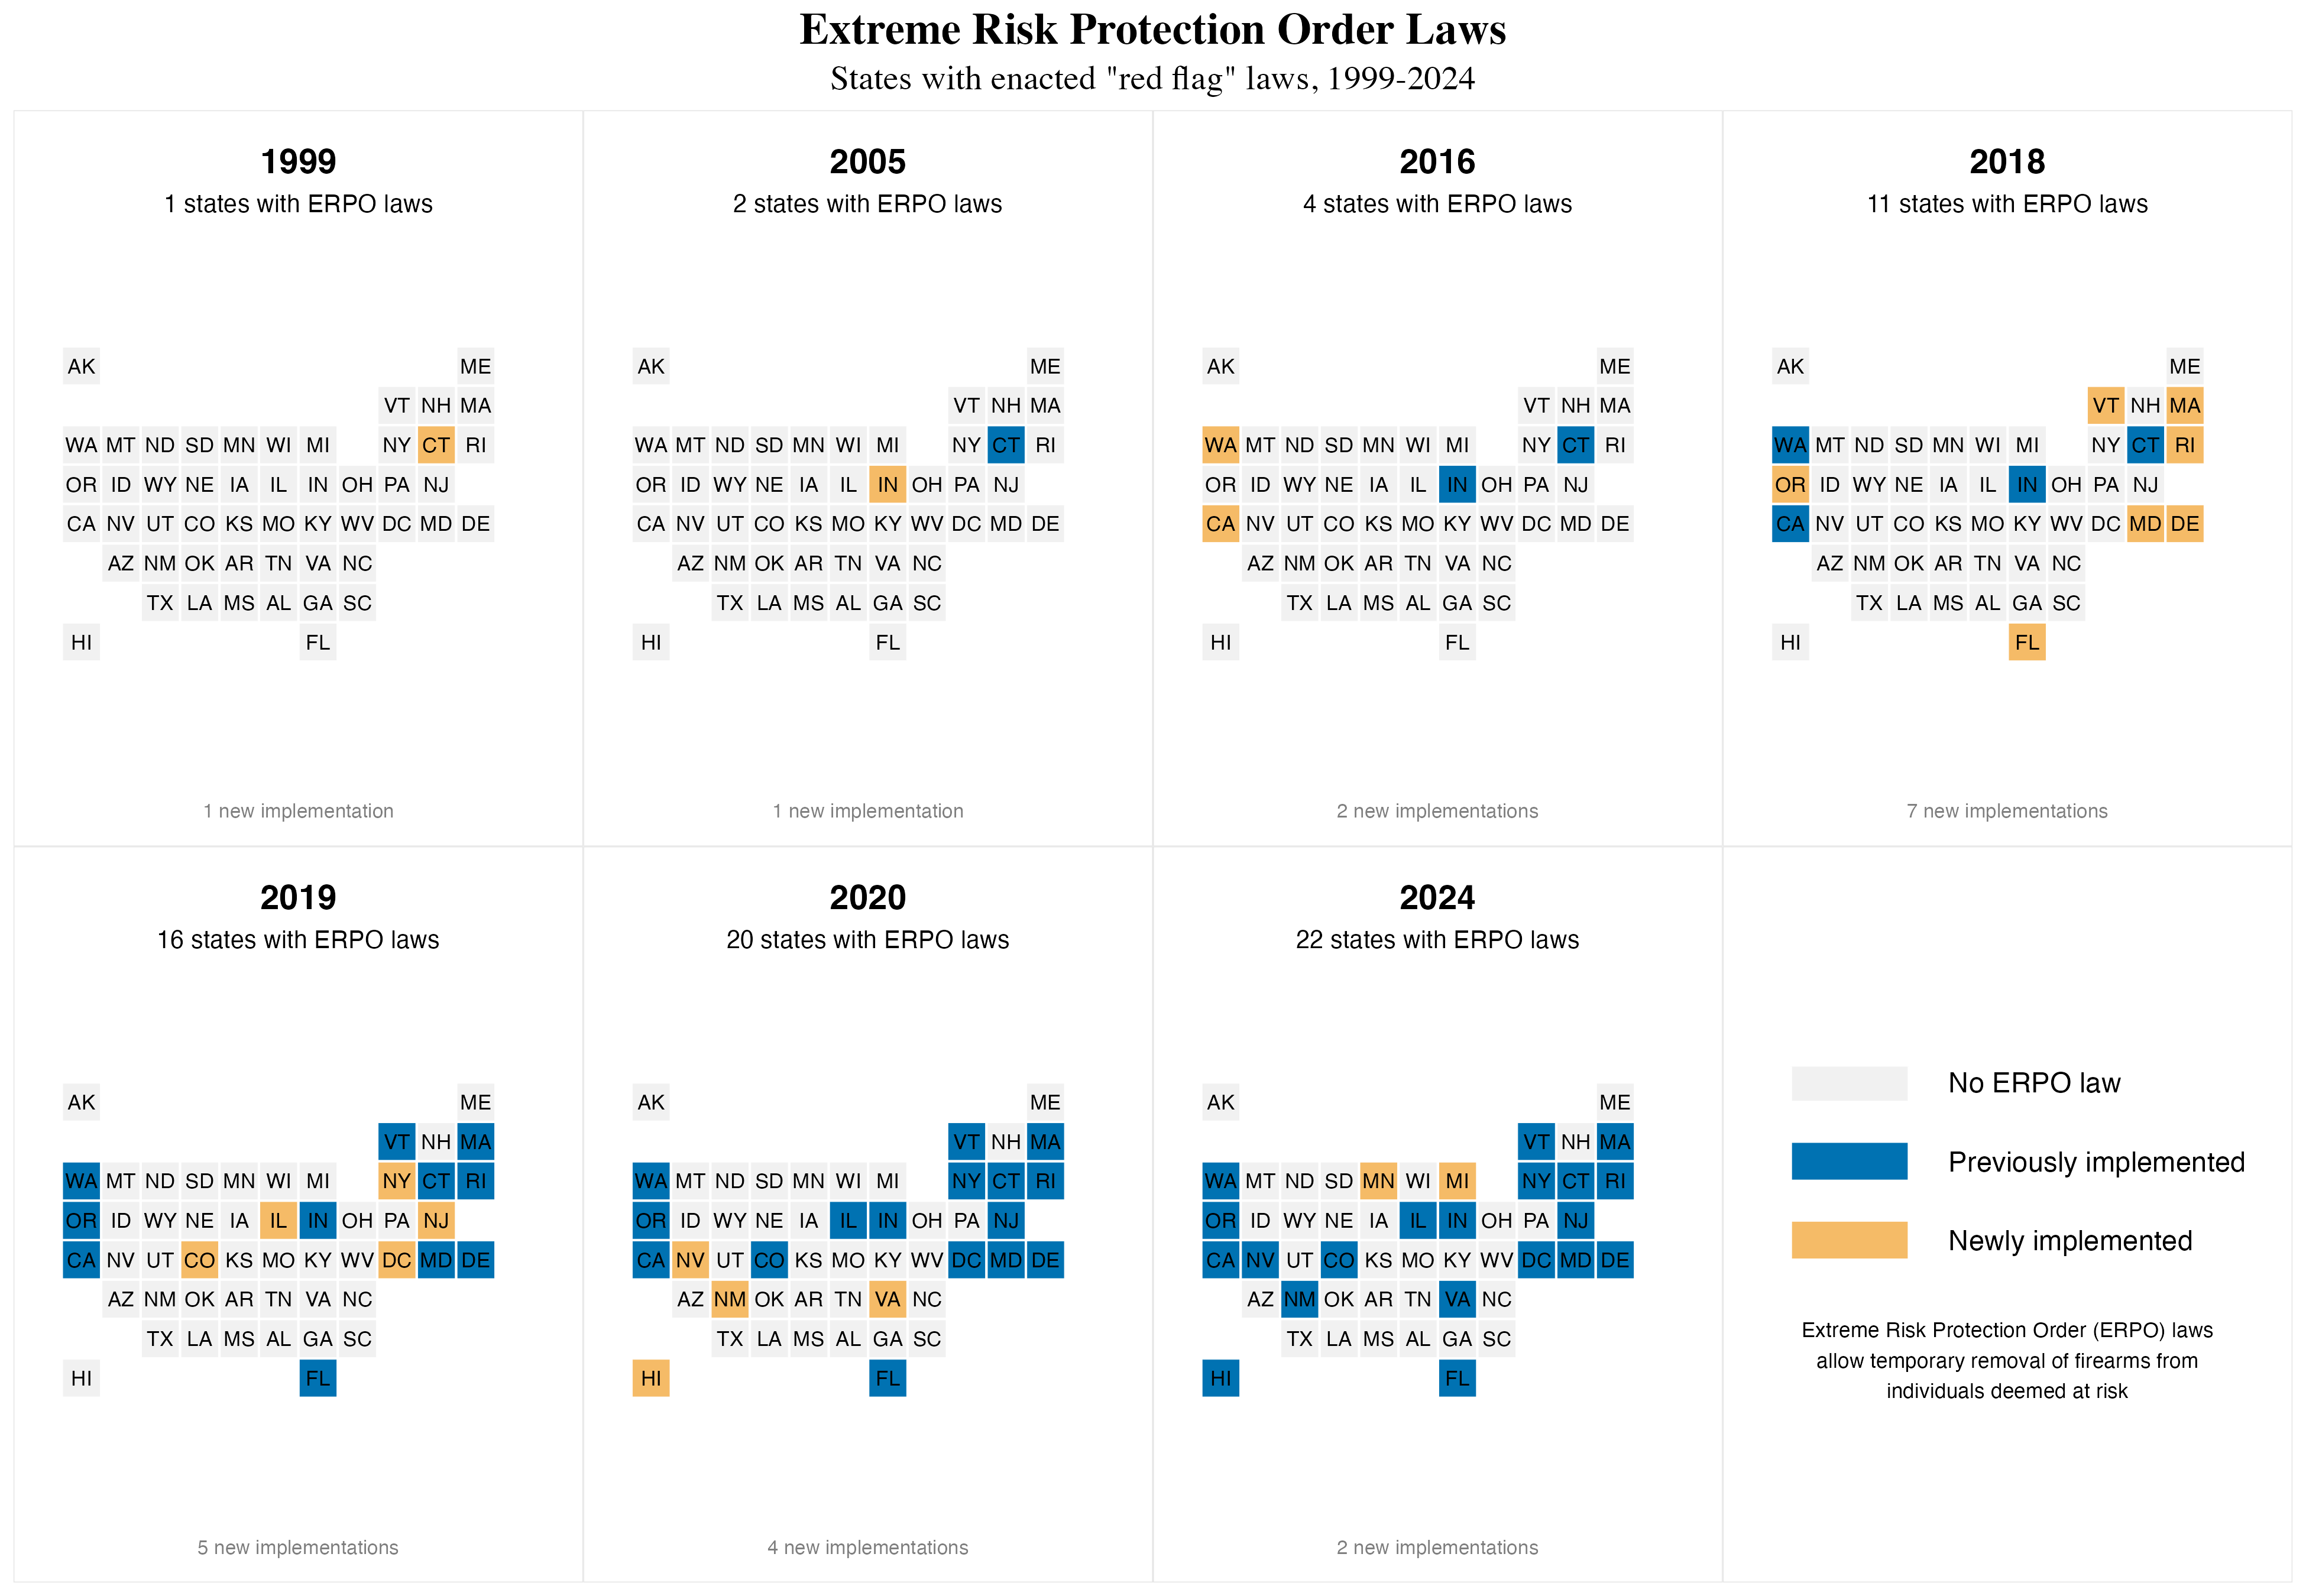
\includegraphics[width=\textwidth]{../erpo_laws_spread.png}
\caption{State Implementation of Extreme Risk Protection Order (ERPO) Laws, 1999–2024}  
\label{fig:erpo_map}
\begin{tablenotes}
\item \footnotesize{\textit{Notes:} This figure shows the annual spread of ERPO laws across U.S. states from 1999 to 2024. States are color-coded by implementation status: orange indicates states that newly implemented an ERPO law in that year, blue indicates states with previously implemented ERPO laws, and gray indicates states without such laws. ERPO laws allow for the temporary removal of firearms from individuals deemed to be at risk of harming themselves or others. By 2024, 22 states had enacted ERPO legislation.}
\end{tablenotes}
\end{figure}

\section{Methods}\label{methods}

The study was determined to be exempt from review and from a requirement
for informed consent, because it used no identifiable human participant
data, by the RAND institutional review board. The study follows good
research practices for comparative effectiveness research,15 eg, the
data sources, modeling methods, primary comparisons, and sensitivity
tests were preregistered, and the data and statistical code are
available. The eAppendix in Supplement 1 provides a detailed discussion
of how the current study extends and improves prior published research
by the authors.

\subsection{Data}\label{data}

Mortality data from 1999 to 2023 come from the National Vital Statistics
System, which provides information on coroners' cause of death
determinations for a near-census of deaths in the United States
\citep[\citet{cdc2024wonder}]{cdc2021wonder}. Information on the
effective dates of firearm laws come from the RAND State Firearm Law
Database.18 The analyses also include state-level demographic, economic,
crime, and gun ownership characteristics; sources for these are
described in the eAppendix in Supplement 1.

\begin{APPENDICES}

\begin{table}[ht]
\centering
\caption{Implementation Timeline of Extreme Risk Protection Order Laws by State (as of April 2024)}
\label{tab:erpo_timeline}
\begin{tabular}{lccc}
\toprule
\textbf{State} & \textbf{Effective Date} & \textbf{Year} & \textbf{Years in Effect (as of 2023)} \\
\midrule
Connecticut & October 1, 1999 & 1999 & 24 \\
Indiana & July 1, 2005 & 2005 & 18 \\
California & January 1, 2016 & 2016 & 7 \\
Washington & December 8, 2016 & 2016 & 7 \\
Oregon & January 1, 2018 & 2018 & 5 \\
Vermont & April 11, 2018 & 2018 & 5 \\
Florida & March 9, 2018 & 2018 & 5 \\
Rhode Island & June 1, 2018 & 2018 & 5 \\
Maryland & October 1, 2018 & 2018 & 5 \\
Massachusetts & August 17, 2018 & 2018 & 5 \\
Delaware & December 27, 2018 & 2018 & 5 \\
Illinois & January 1, 2019 & 2019 & 4 \\
Colorado & April 12, 2019 & 2019 & 4 \\
District of Columbia & January 30, 2019 & 2019 & 4 \\
New York & August 24, 2019 & 2019 & 4 \\
New Jersey & September 1, 2019 & 2019 & 4 \\
Hawaii & January 1, 2020 & 2020 & 3 \\
Nevada & January 1, 2020 & 2020 & 3 \\
New Mexico & May 20, 2020 & 2020 & 3 \\
Virginia & July 1, 2020 & 2020 & 3 \\
U.S. Virgin Islands & February 1, 2023 & 2023 & <1 \\
Michigan & February 13, 2024 & 2024 & 0 \\
Minnesota & January 1, 2024 & 2024 & 0 \\
\bottomrule
\multicolumn{4}{p{.97\linewidth}}{\small \textit{Sources:} RAND State Firearm Law Database (2024); Johns Hopkins Center for Gun Violence Solutions (2023); Giffords Law Center (2023).}
\end{tabular}
\end{table}

\clearpage

\begin{table}[ht]
\centering
\caption{Key Policy Features of Extreme Risk Protection Order Laws (as of April 2024)}
\label{tab:erpo_features}
\begin{tabular}{lcccccc}
\toprule
\multirow{2}{*}{\textbf{State}} & \multicolumn{3}{c}{\textbf{Authorized Petitioners}} & \multicolumn{2}{c}{\textbf{Ex Parte Provisions}} & \multirow{2}{*}{\textbf{Final Order}} \\
\cmidrule(lr){2-4} \cmidrule(lr){5-6}
 & \textbf{Law Enf.} & \textbf{Family} & \textbf{Other} & \textbf{Available} & \textbf{Duration (days)} & \textbf{Duration} \\
\midrule
California & \checkmark & \checkmark & \checkmark & \checkmark & 21 & 1-5 years \\
Colorado & \checkmark & \checkmark & \checkmark & \checkmark & 14 & 364 days \\
Connecticut & \checkmark & \checkmark & \checkmark & \checkmark & 14 & Until terminated \\
Delaware & \checkmark & \checkmark & - & \checkmark & 15 & Up to 1 year \\
District of Columbia & \checkmark & \checkmark & \checkmark & \checkmark & 14 & 1 year \\
Florida & \checkmark & - & - & \checkmark & 14 & Up to 1 year \\
Hawaii & \checkmark & \checkmark & \checkmark & \checkmark & 14 & 1 year \\
Illinois & \checkmark & \checkmark & - & \checkmark & 14 & 6 mo. to 1 yr. \\
Indiana & \checkmark & - & - & \checkmark & 14 & Until terminated \\
Maryland & \checkmark & \checkmark & \checkmark & \checkmark & 7 & Up to 1 year \\
Massachusetts & \checkmark & \checkmark & \checkmark & \checkmark & 10 & Up to 1 year \\
Michigan & \checkmark & \checkmark & \checkmark & \checkmark & 14 & 1 year \\
Minnesota & \checkmark & \checkmark & \checkmark & \checkmark & 14 & 6 mo. to 1 yr. \\
Nevada & \checkmark & \checkmark & - & \checkmark & 7 & Up to 1 year \\
New Jersey & \checkmark & \checkmark & - & \checkmark & 10 & Until terminated \\
New Mexico & \checkmark & - & - & \checkmark & 10 & Up to 1 year \\
New York & \checkmark & \checkmark & \checkmark & \checkmark & 6 & Up to 1 year \\
Oregon & \checkmark & \checkmark & - & - & N/A & 1 year \\
Rhode Island & \checkmark & - & - & \checkmark & 14 & 1 year \\
U.S. Virgin Islands & \checkmark & \checkmark & \checkmark & \checkmark & 14 & 1 year \\
Vermont & \checkmark & \checkmark & - & \checkmark & 14 & Up to 6 months \\
Virginia & \checkmark & \checkmark & - & \checkmark & 14 & Up to 180 days \\
Washington & \checkmark & \checkmark & - & \checkmark & 14 & 1 year \\
\bottomrule
\multicolumn{7}{p{.97\linewidth}}{\small \textit{Notes:} "Other" petitioners may include healthcare professionals, educators, co-workers, or state's attorneys, depending on the state. "Law Enf." refers to law enforcement officers. Michigan and Minnesota laws went into effect in 2024.}
\end{tabular}
\end{table}

\clearpage

\begin{table}[ht]
\centering
\caption{Classification of ERPO Laws by Policy Feature Categories (as of April 2024)}
\label{tab:erpo_categories}
\begin{tabular}{lcc}
\toprule
\textbf{Policy Feature} & \textbf{States} & \textbf{Count} \\
\midrule
\textbf{Petitioner Access} & & \\
Law Enforcement Only & Florida, Indiana, New Mexico, Rhode Island & 4 \\
Family Members Included & All other ERPO states & 19 \\
Healthcare Prof. Included & CA, CO, CT, DC, HI, MD, MA, MI, MN, NY, VI & 11 \\
\midrule
\textbf{Ex Parte Provisions} & & \\
Available & All except Oregon & 22 \\
Not Available & Oregon & 1 \\
Short Duration ($\leq$10 days) & MD, MA, NJ, NM, NY, NV & 6 \\
Standard Duration (>10 days) & All others with ex parte & 16 \\
\midrule
\textbf{Final Order Duration} & & \\
6 months or less & Vermont, Virginia & 2 \\
Up to 1 year (standard) & Most states & 18 \\
Until terminated & Connecticut, Indiana, New Jersey & 3 \\
\midrule
\textbf{Implementation Intensity} & & \\
High & Florida, Maryland & 2 \\
Medium & CA, CO, CT, NY, OR, RI, WA & 7 \\
Low & All others & 14 \\
\bottomrule
\multicolumn{3}{p{.95\linewidth}}{\small \textit{Sources:} Data compiled from Johns Hopkins Center for Gun Violence Solutions (2023), RAND State Firearm Law Database (2024), and Giffords Law Center (2023). Implementation intensity categories based on estimated ERPOs per 100,000 population.}
\end{tabular}
\end{table}

If there is more than one appendix (i.e., several unrelated sections),
one should use \texttt{APPENDICES} instead, and add section headings
like this.

\section{Section A}\label{section-a}

Content

\section{Section B}\label{section-b}

Content

\end{APPENDICES}

% Appendix here
% Options are (1) APPENDIX (with or without general title) or
%             (2) APPENDICES (if it has more than one unrelated sections)
% Outcomment the appropriate case if necessary
%
% \begin{APPENDIX}{<Title of the Appendix>}
% \end{APPENDIX}
%
%   or
%
% \begin{APPENDICES}
% \section{<Title of Section A>}
% \section{<Title of Section B>}
% etc
% \end{APPENDICES}


% Acknowledgments here
\ACKNOWLEDGMENT{The author would like to thank colleagues at the Harvard
Kennedy School and members of the CAUSALab and PIAS-Lab for their
insights and support throughout this project.}

\bibliographystyle{informs2014}
\bibliography{references.bib}



\end{document}
